\documentclass[11pt]{article}
\usepackage[textwidth=18.0cm, textheight=23.0cm, top=2.0cm]{geometry}
\usepackage{pst-all}
\usepackage{amssymb}
\usepackage{tikz}
\usepackage{underscore}\begin{document}
\pagestyle{empty}


ClassName: \underline{\textbf{Class_10.2bp-28}}
\par
BinSize: \underline{\textbf{100 × 100}}
\par
ReduceSize: \underline{\textbf{100 × 100}}
\par
TypeNum: \underline{\textbf{60}}
\par
Num: \underline{\textbf{60}}
\par
OutS: \underline{\textbf{90000}}
\par
InS: \underline{\textbf{79106}}
\par
Rate: \underline{\textbf{0.879}}
\par
UB: \underline{\textbf{9}}
\par
LB0: \underline{\textbf{8}}
\par
LB: \underline{\textbf{9}}
\par
LBWithCut: \underline{\textbf{9}}
\par
NodeCut: \underline{\textbf{0}}
\par
ExtendedNodeCnt: \underline{\textbf{1}}
\par
GenNodeCnt: \underline{\textbf{1}}
\par
PrimalNode: \underline{\textbf{0}}
\par
ColumnCount: \underline{\textbf{60}}
\par
TotalCutCount: \underline{\textbf{0}}
\par
RootCutCount: \underline{\textbf{0}}
\par
LPSolverCnt: \underline{\textbf{52}}
\par
PricingSolverCnt: \underline{\textbf{52}}
\par
BranchAndBoundNum: \underline{\textbf{1}}
\par
isOpt: \underline{\textbf{false}}
\par
TimeOnInitSolution: \underline{\textbf{600.000 s}}
\par
TimeOnPrimal: \underline{\textbf{0.000 s}}
\par
TimeOnPricing: \underline{\textbf{2999.665 s}}
\par
TimeOnRmp: \underline{\textbf{0.081 s}}
\par
TotalTime: \underline{\textbf{3599.997 s}}
\par
\newpage


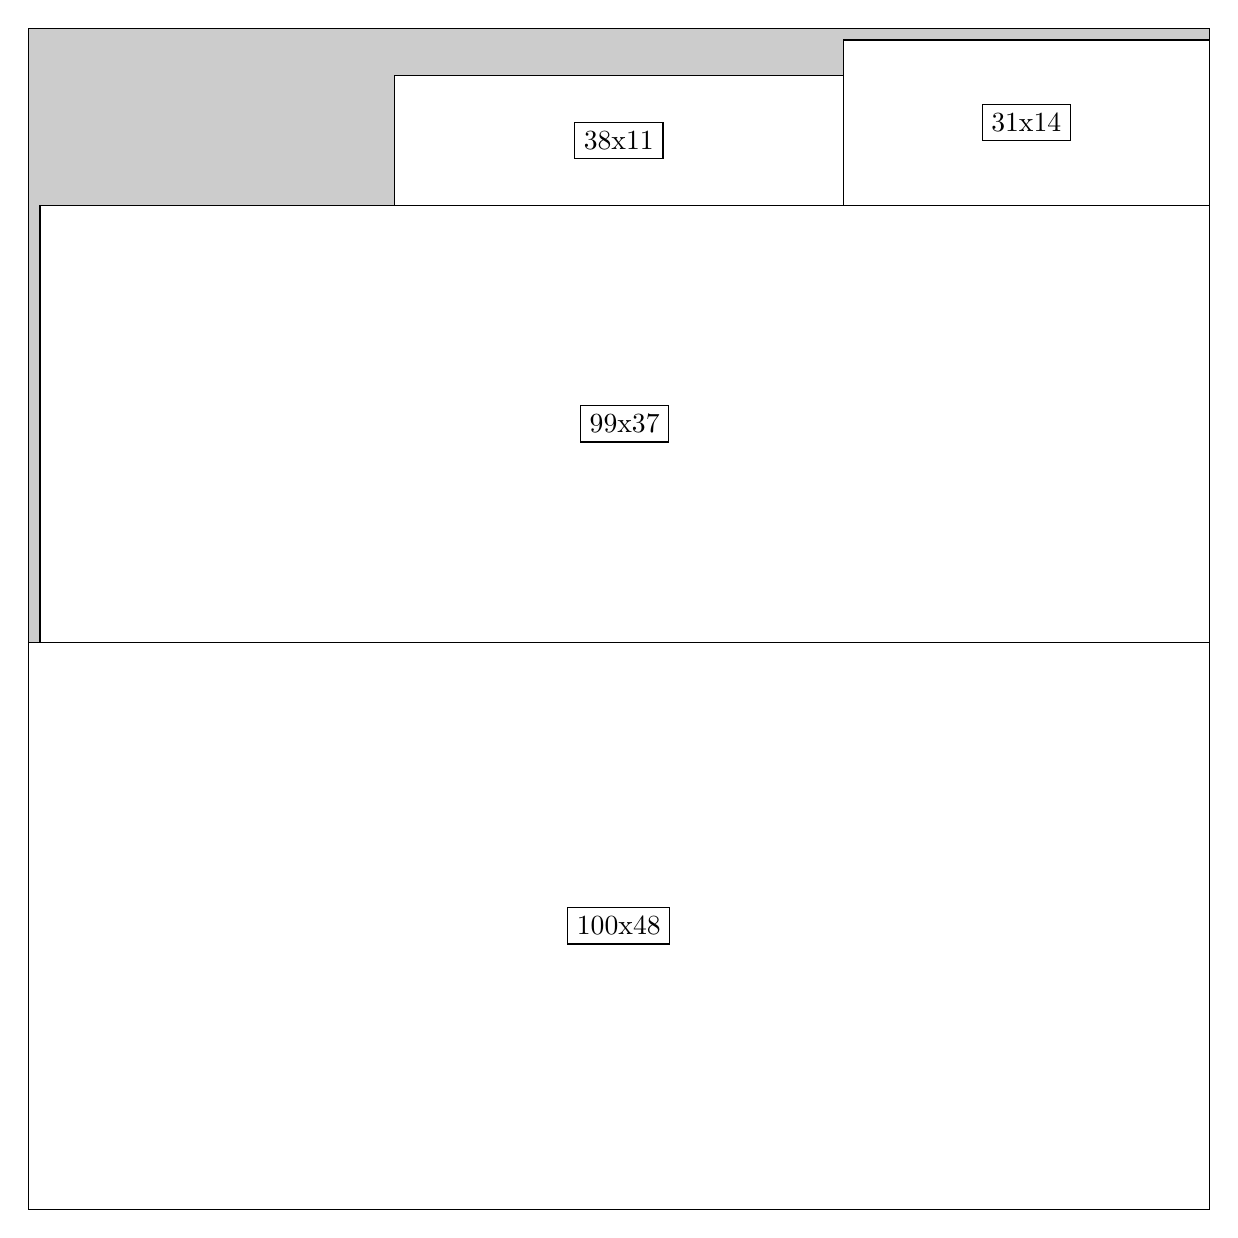
\begin{tikzpicture}[shorten >=1pt,scale=1.0,every node/.style={scale=1.0},->]
\tikzstyle{vertex}=[circle,fill=black!25,minimum size=14pt,inner sep=0pt]
\filldraw[fill=gray!40!white, draw=black] (0,0) rectangle (15.0,15.0);
\foreach \name/\x/\y/\w/\h in {100x48/0.0/0.0/15.0/7.199999999999999,99x37/0.15/7.199999999999999/14.85/5.55,31x14/10.35/12.75/4.6499999999999995/2.1,38x11/4.6499999999999995/12.75/5.7/1.65}
\filldraw[fill=white!40!white, draw=black] (\x,\y) rectangle node[draw] (\name) {\name} ++(\w,\h);
\end{tikzpicture}


w =100 , h =48 , x =0 , y =0 , v =4800
\par
w =99 , h =37 , x =1 , y =48 , v =3663
\par
w =31 , h =14 , x =69 , y =85 , v =434
\par
w =38 , h =11 , x =31 , y =85 , v =418
\par
\newpage


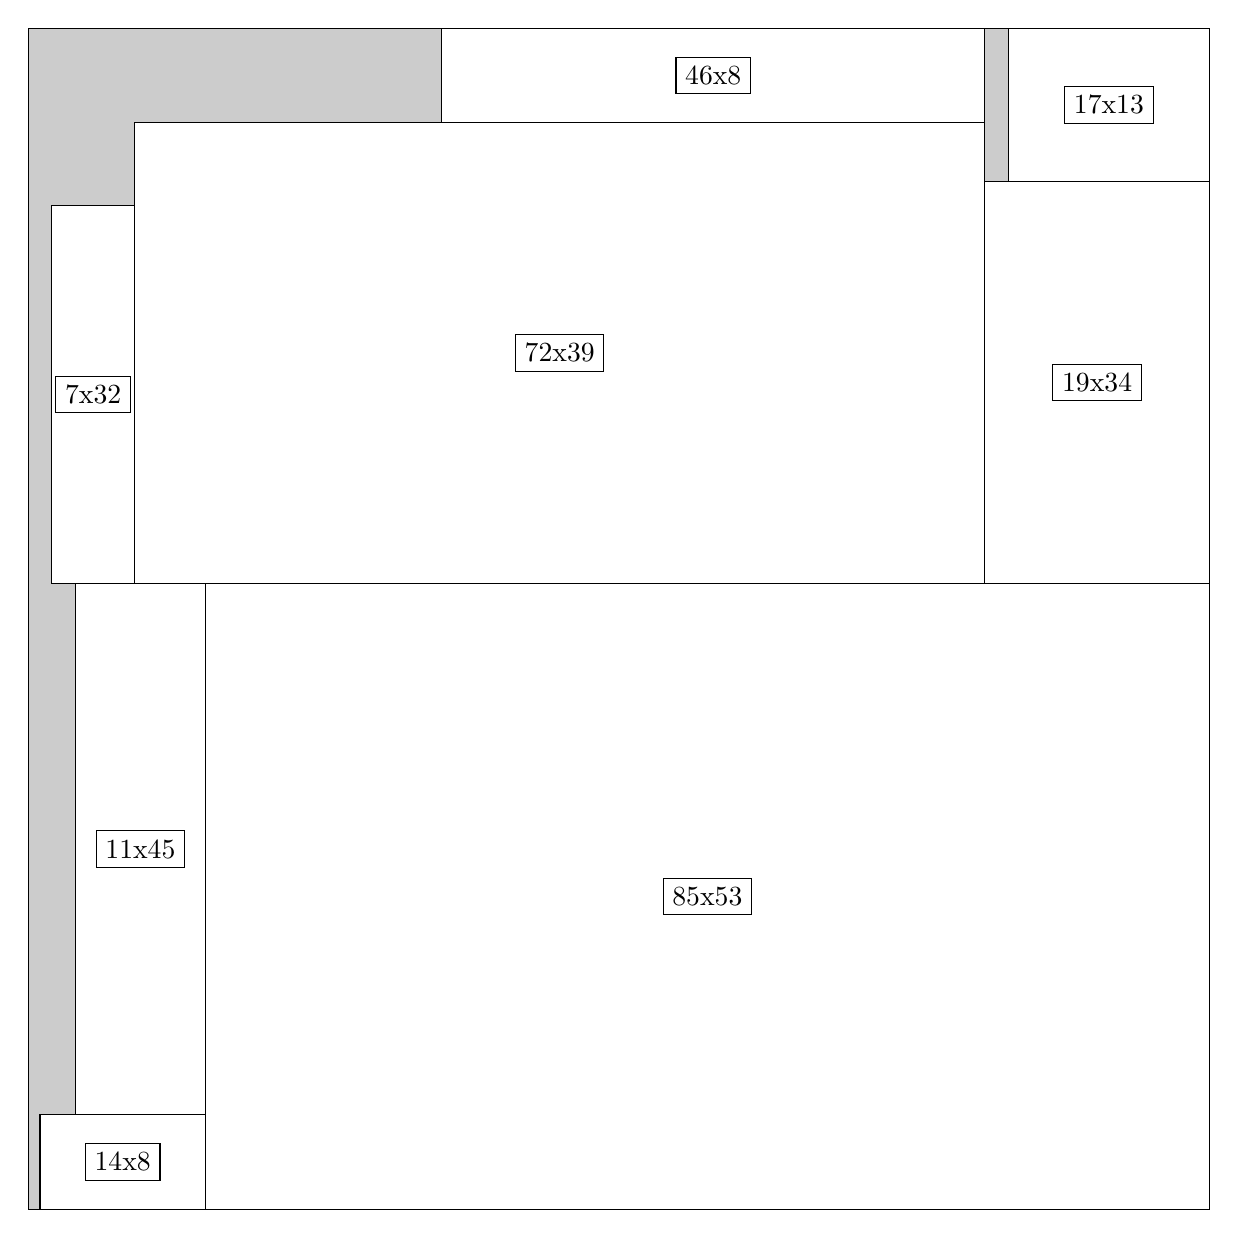
\begin{tikzpicture}[shorten >=1pt,scale=1.0,every node/.style={scale=1.0},->]
\tikzstyle{vertex}=[circle,fill=black!25,minimum size=14pt,inner sep=0pt]
\filldraw[fill=gray!40!white, draw=black] (0,0) rectangle (15.0,15.0);
\foreach \name/\x/\y/\w/\h in {85x53/2.25/0.0/12.75/7.949999999999999,14x8/0.15/0.0/2.1/1.2,11x45/0.6/1.2/1.65/6.75,19x34/12.15/7.949999999999999/2.85/5.1,17x13/12.45/13.049999999999999/2.55/1.95,72x39/1.3499999999999999/7.949999999999999/10.799999999999999/5.85,46x8/5.25/13.799999999999999/6.8999999999999995/1.2,7x32/0.3/7.949999999999999/1.05/4.8}
\filldraw[fill=white!40!white, draw=black] (\x,\y) rectangle node[draw] (\name) {\name} ++(\w,\h);
\end{tikzpicture}


w =85 , h =53 , x =15 , y =0 , v =4505
\par
w =14 , h =8 , x =1 , y =0 , v =112
\par
w =11 , h =45 , x =4 , y =8 , v =495
\par
w =19 , h =34 , x =81 , y =53 , v =646
\par
w =17 , h =13 , x =83 , y =87 , v =221
\par
w =72 , h =39 , x =9 , y =53 , v =2808
\par
w =46 , h =8 , x =35 , y =92 , v =368
\par
w =7 , h =32 , x =2 , y =53 , v =224
\par
\newpage


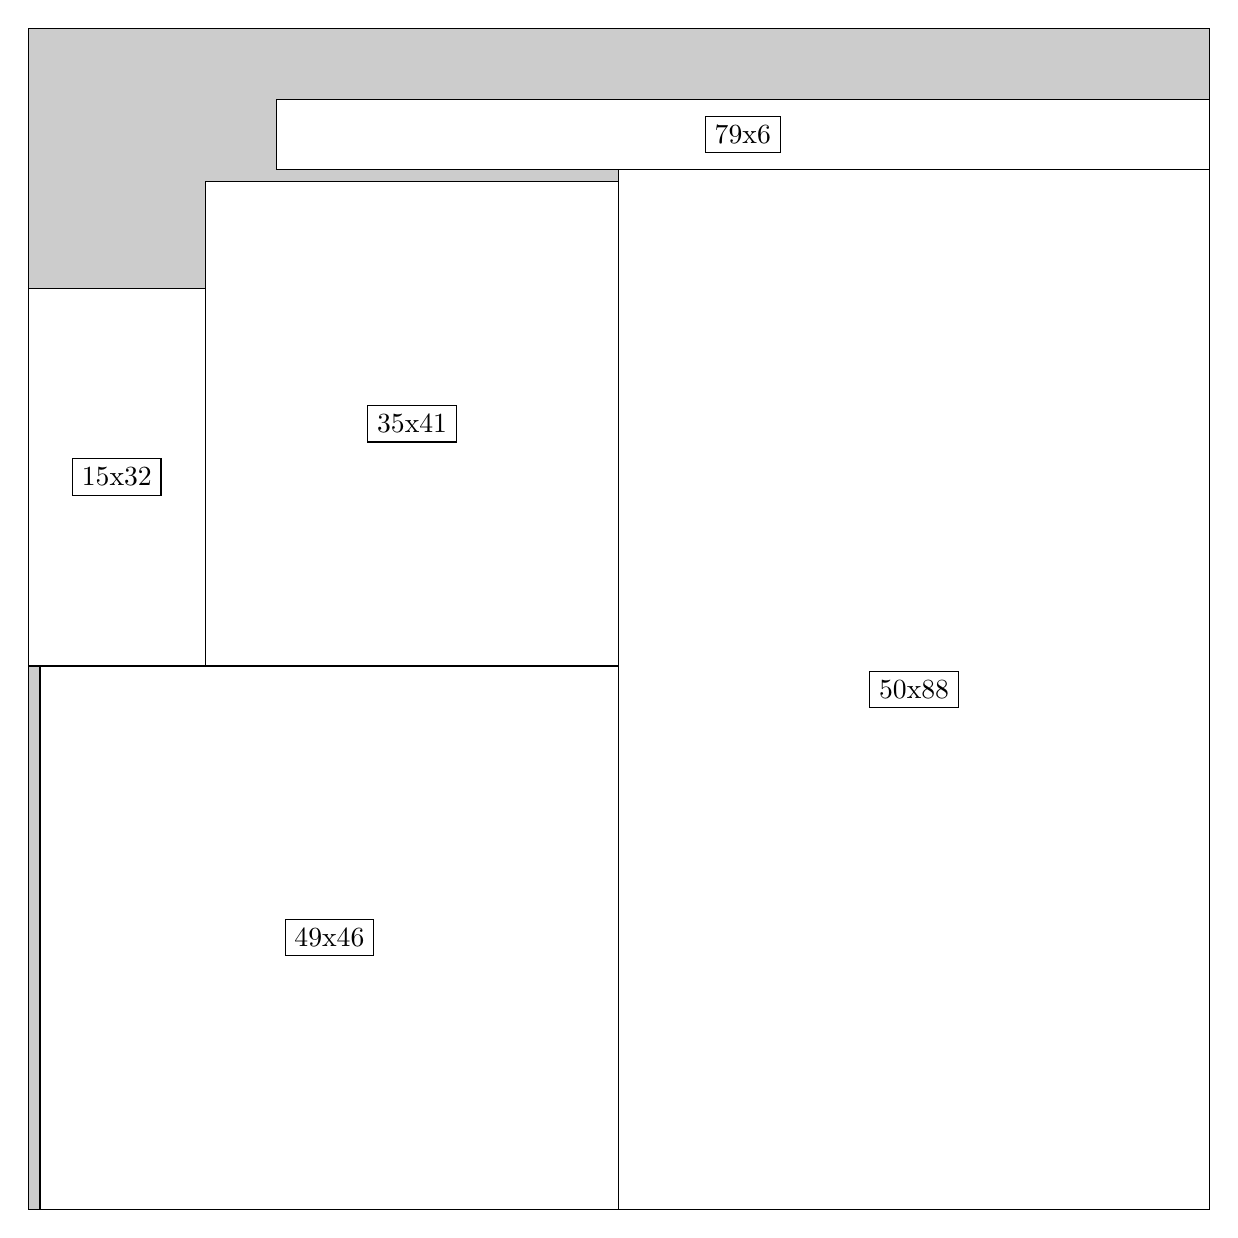
\begin{tikzpicture}[shorten >=1pt,scale=1.0,every node/.style={scale=1.0},->]
\tikzstyle{vertex}=[circle,fill=black!25,minimum size=14pt,inner sep=0pt]
\filldraw[fill=gray!40!white, draw=black] (0,0) rectangle (15.0,15.0);
\foreach \name/\x/\y/\w/\h in {50x88/7.5/0.0/7.5/13.2,49x46/0.15/0.0/7.35/6.8999999999999995,35x41/2.25/6.8999999999999995/5.25/6.1499999999999995,15x32/0.0/6.8999999999999995/2.25/4.8,79x6/3.15/13.2/11.85/0.8999999999999999}
\filldraw[fill=white!40!white, draw=black] (\x,\y) rectangle node[draw] (\name) {\name} ++(\w,\h);
\end{tikzpicture}


w =50 , h =88 , x =50 , y =0 , v =4400
\par
w =49 , h =46 , x =1 , y =0 , v =2254
\par
w =35 , h =41 , x =15 , y =46 , v =1435
\par
w =15 , h =32 , x =0 , y =46 , v =480
\par
w =79 , h =6 , x =21 , y =88 , v =474
\par
\newpage


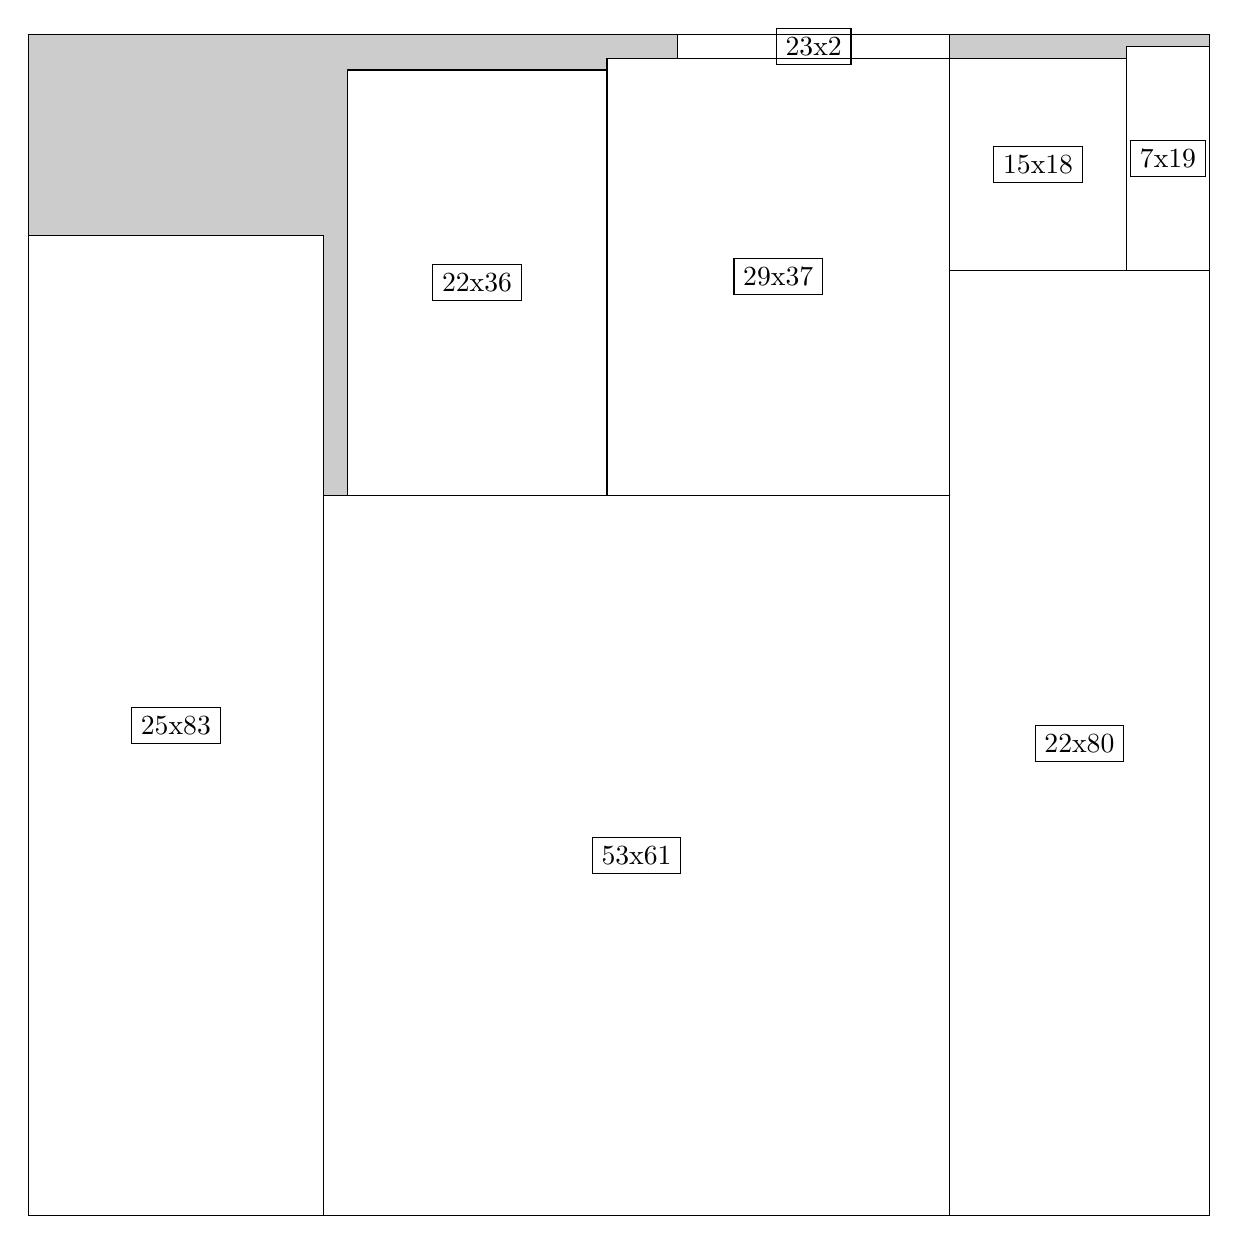
\begin{tikzpicture}[shorten >=1pt,scale=1.0,every node/.style={scale=1.0},->]
\tikzstyle{vertex}=[circle,fill=black!25,minimum size=14pt,inner sep=0pt]
\filldraw[fill=gray!40!white, draw=black] (0,0) rectangle (15.0,15.0);
\foreach \name/\x/\y/\w/\h in {22x80/11.7/0.0/3.3/12.0,7x19/13.95/12.0/1.05/2.85,15x18/11.7/12.0/2.25/2.6999999999999997,53x61/3.75/0.0/7.949999999999999/9.15,29x37/7.35/9.15/4.35/5.55,23x2/8.25/14.7/3.4499999999999997/0.3,22x36/4.05/9.15/3.3/5.3999999999999995,25x83/0.0/0.0/3.75/12.45}
\filldraw[fill=white!40!white, draw=black] (\x,\y) rectangle node[draw] (\name) {\name} ++(\w,\h);
\end{tikzpicture}


w =22 , h =80 , x =78 , y =0 , v =1760
\par
w =7 , h =19 , x =93 , y =80 , v =133
\par
w =15 , h =18 , x =78 , y =80 , v =270
\par
w =53 , h =61 , x =25 , y =0 , v =3233
\par
w =29 , h =37 , x =49 , y =61 , v =1073
\par
w =23 , h =2 , x =55 , y =98 , v =46
\par
w =22 , h =36 , x =27 , y =61 , v =792
\par
w =25 , h =83 , x =0 , y =0 , v =2075
\par
\newpage


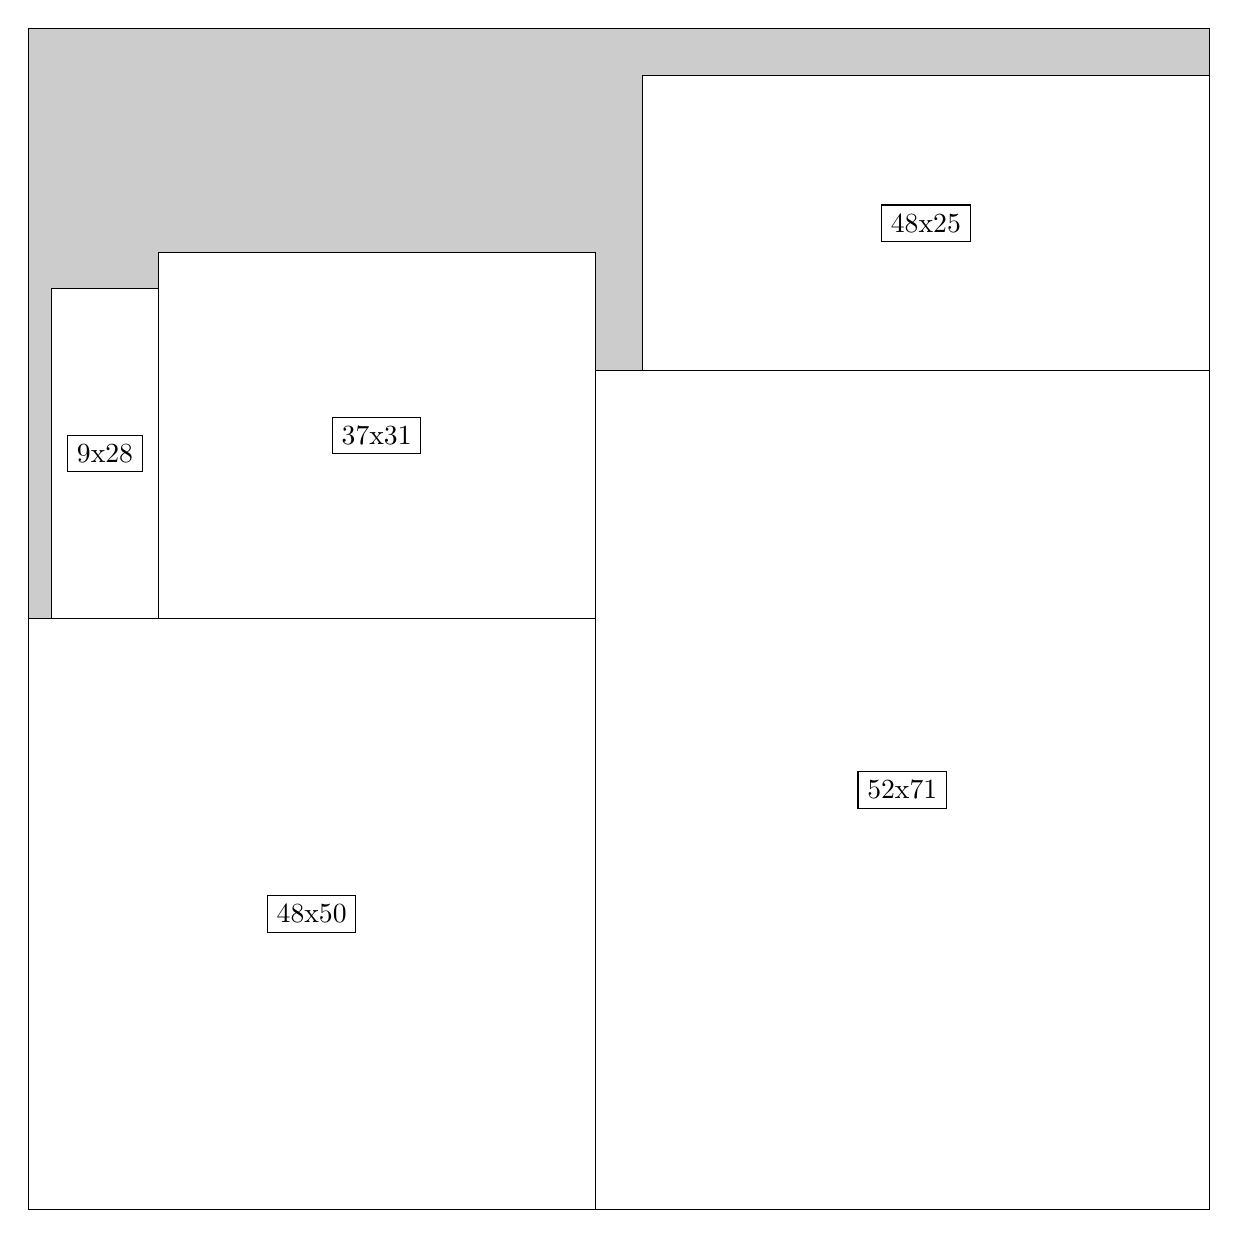
\begin{tikzpicture}[shorten >=1pt,scale=1.0,every node/.style={scale=1.0},->]
\tikzstyle{vertex}=[circle,fill=black!25,minimum size=14pt,inner sep=0pt]
\filldraw[fill=gray!40!white, draw=black] (0,0) rectangle (15.0,15.0);
\foreach \name/\x/\y/\w/\h in {52x71/7.199999999999999/0.0/7.8/10.65,48x25/7.8/10.65/7.199999999999999/3.75,48x50/0.0/0.0/7.199999999999999/7.5,37x31/1.65/7.5/5.55/4.6499999999999995,9x28/0.3/7.5/1.3499999999999999/4.2}
\filldraw[fill=white!40!white, draw=black] (\x,\y) rectangle node[draw] (\name) {\name} ++(\w,\h);
\end{tikzpicture}


w =52 , h =71 , x =48 , y =0 , v =3692
\par
w =48 , h =25 , x =52 , y =71 , v =1200
\par
w =48 , h =50 , x =0 , y =0 , v =2400
\par
w =37 , h =31 , x =11 , y =50 , v =1147
\par
w =9 , h =28 , x =2 , y =50 , v =252
\par
\newpage


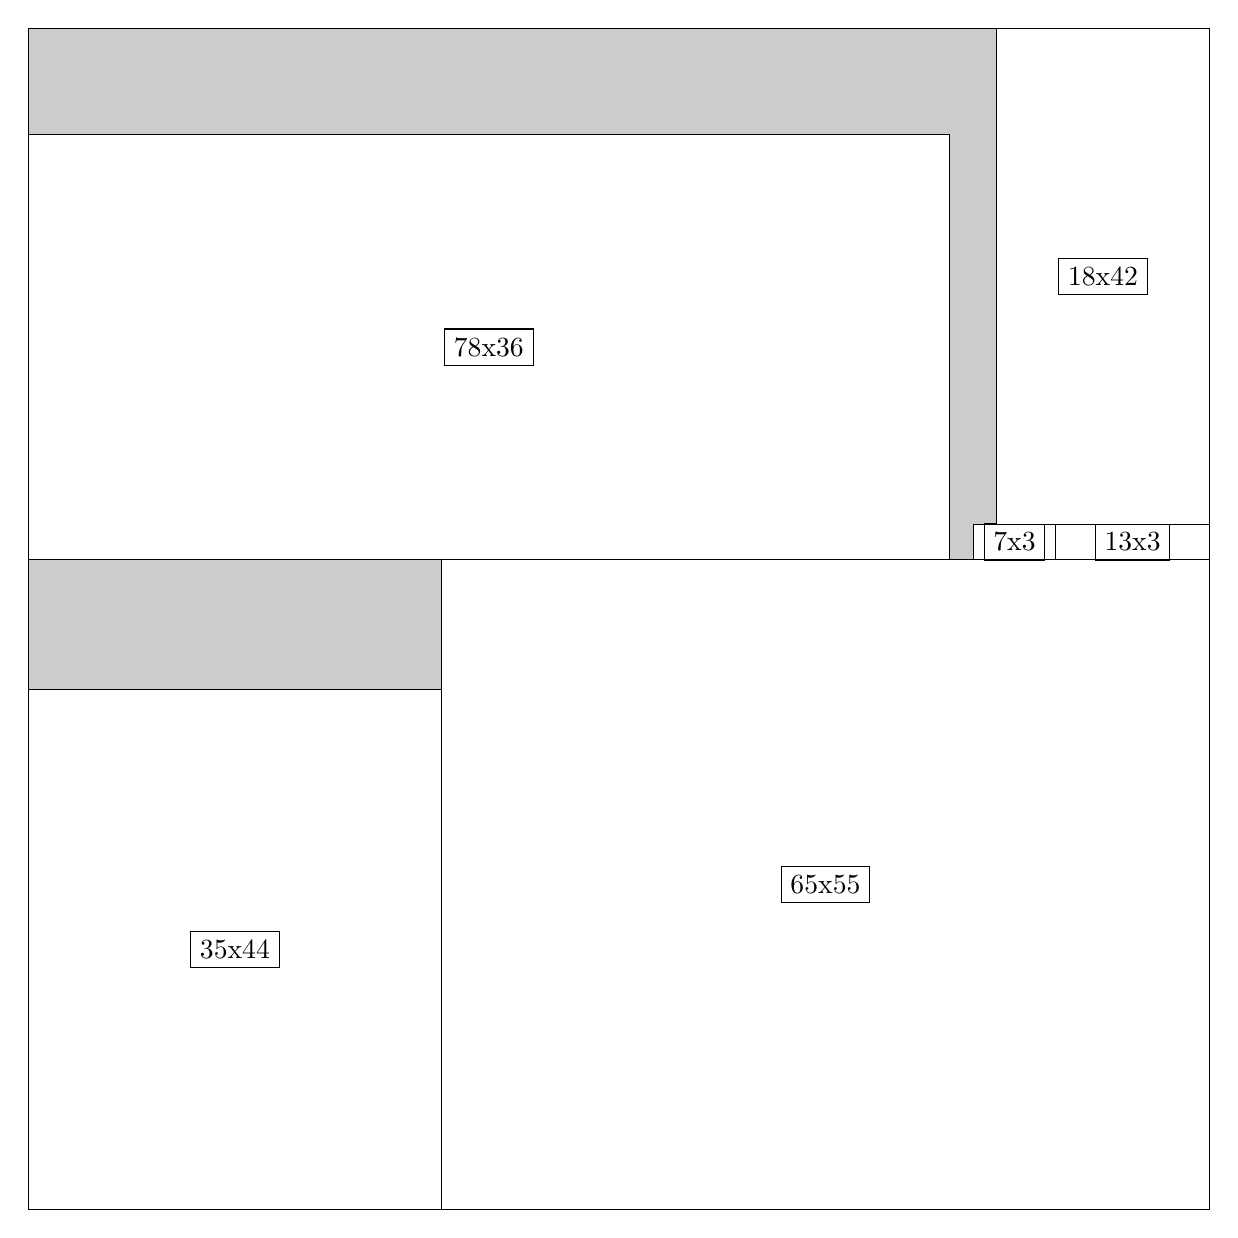
\begin{tikzpicture}[shorten >=1pt,scale=1.0,every node/.style={scale=1.0},->]
\tikzstyle{vertex}=[circle,fill=black!25,minimum size=14pt,inner sep=0pt]
\filldraw[fill=gray!40!white, draw=black] (0,0) rectangle (15.0,15.0);
\foreach \name/\x/\y/\w/\h in {65x55/5.25/0.0/9.75/8.25,35x44/0.0/0.0/5.25/6.6,13x3/13.049999999999999/8.25/1.95/0.44999999999999996,7x3/12.0/8.25/1.05/0.44999999999999996,18x42/12.299999999999999/8.7/2.6999999999999997/6.3,78x36/0.0/8.25/11.7/5.3999999999999995}
\filldraw[fill=white!40!white, draw=black] (\x,\y) rectangle node[draw] (\name) {\name} ++(\w,\h);
\end{tikzpicture}


w =65 , h =55 , x =35 , y =0 , v =3575
\par
w =35 , h =44 , x =0 , y =0 , v =1540
\par
w =13 , h =3 , x =87 , y =55 , v =39
\par
w =7 , h =3 , x =80 , y =55 , v =21
\par
w =18 , h =42 , x =82 , y =58 , v =756
\par
w =78 , h =36 , x =0 , y =55 , v =2808
\par
\newpage


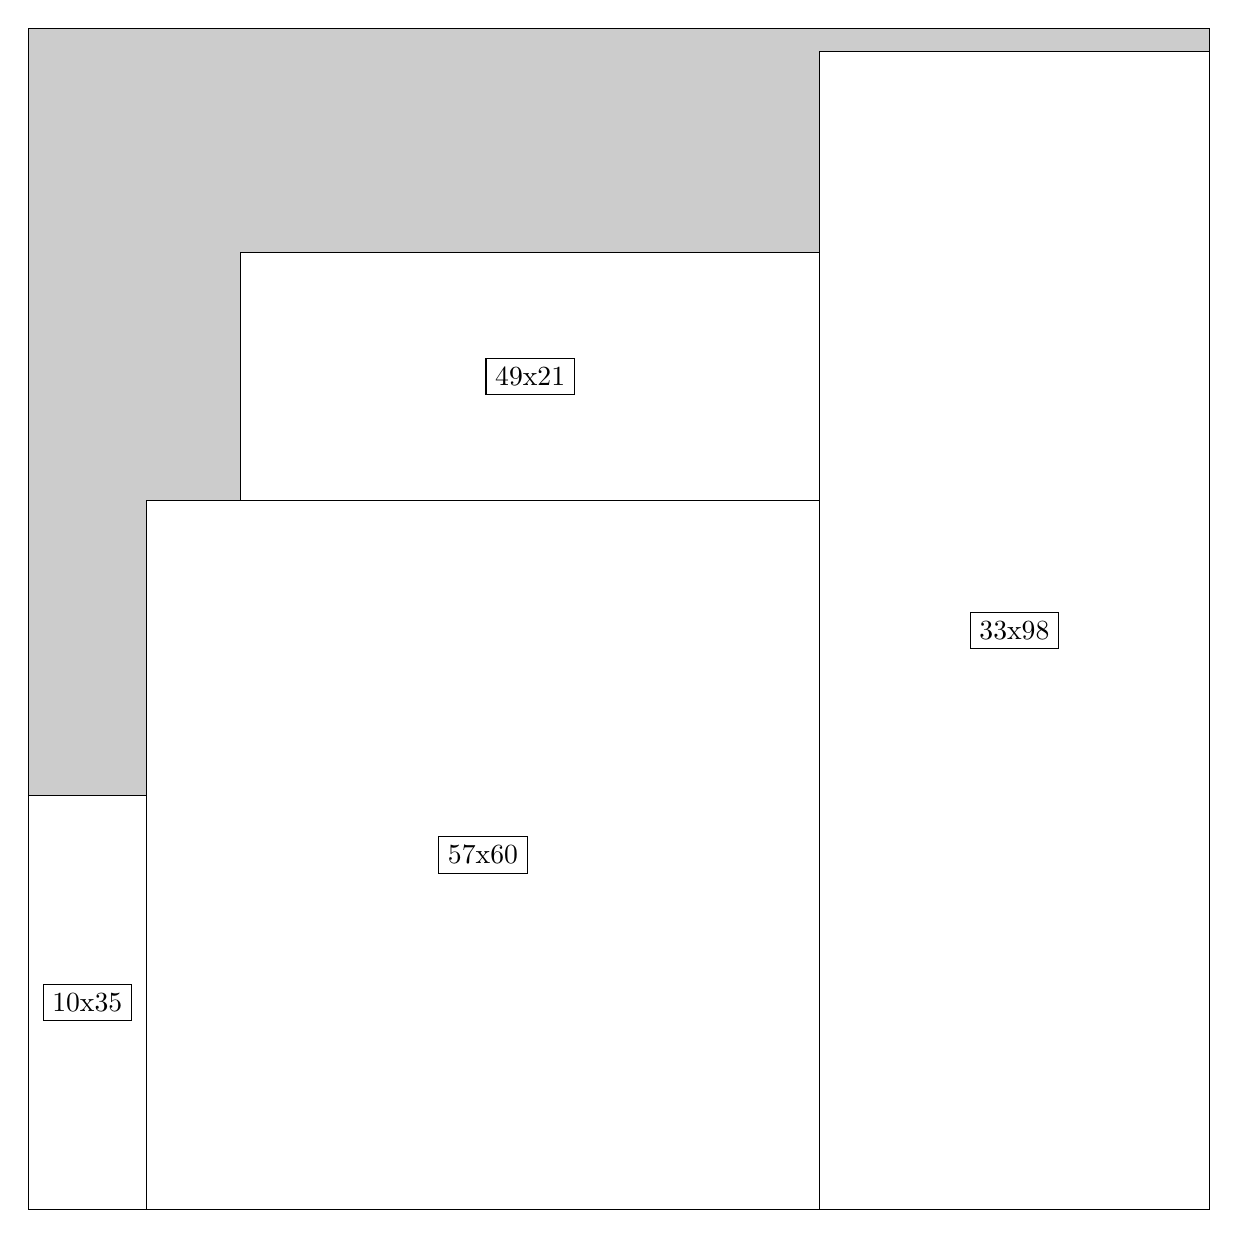
\begin{tikzpicture}[shorten >=1pt,scale=1.0,every node/.style={scale=1.0},->]
\tikzstyle{vertex}=[circle,fill=black!25,minimum size=14pt,inner sep=0pt]
\filldraw[fill=gray!40!white, draw=black] (0,0) rectangle (15.0,15.0);
\foreach \name/\x/\y/\w/\h in {33x98/10.049999999999999/0.0/4.95/14.7,57x60/1.5/0.0/8.549999999999999/9.0,49x21/2.6999999999999997/9.0/7.35/3.15,10x35/0.0/0.0/1.5/5.25}
\filldraw[fill=white!40!white, draw=black] (\x,\y) rectangle node[draw] (\name) {\name} ++(\w,\h);
\end{tikzpicture}


w =33 , h =98 , x =67 , y =0 , v =3234
\par
w =57 , h =60 , x =10 , y =0 , v =3420
\par
w =49 , h =21 , x =18 , y =60 , v =1029
\par
w =10 , h =35 , x =0 , y =0 , v =350
\par
\newpage


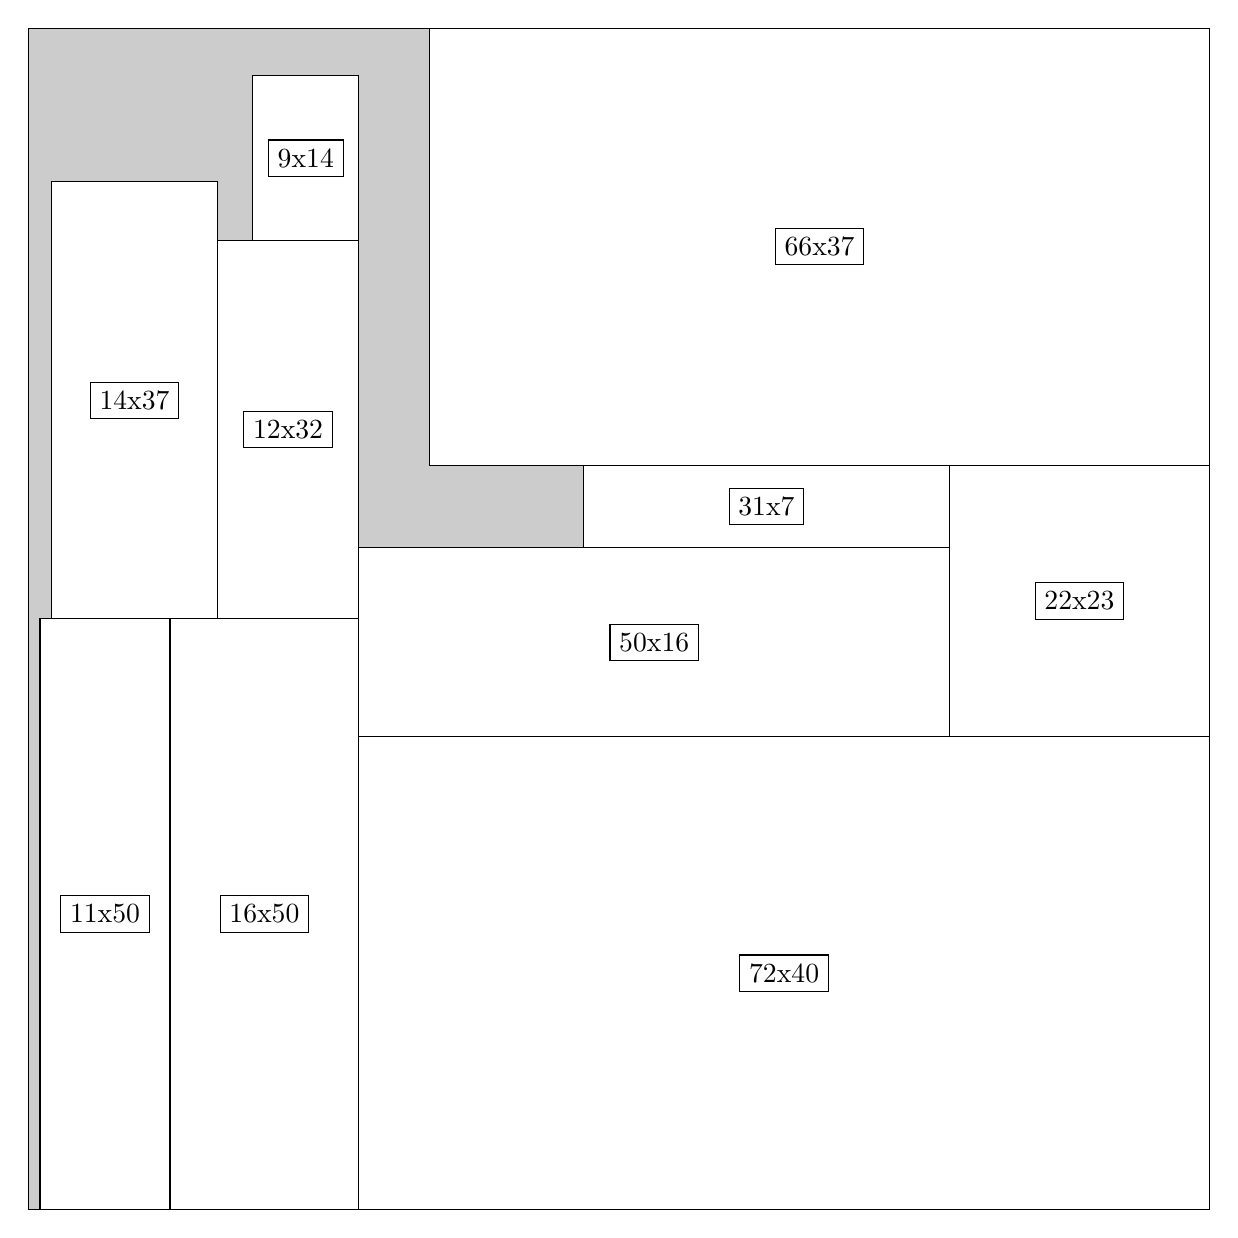
\begin{tikzpicture}[shorten >=1pt,scale=1.0,every node/.style={scale=1.0},->]
\tikzstyle{vertex}=[circle,fill=black!25,minimum size=14pt,inner sep=0pt]
\filldraw[fill=gray!40!white, draw=black] (0,0) rectangle (15.0,15.0);
\foreach \name/\x/\y/\w/\h in {72x40/4.2/0.0/10.799999999999999/6.0,22x23/11.7/6.0/3.3/3.4499999999999997,50x16/4.2/6.0/7.5/2.4,31x7/7.05/8.4/4.6499999999999995/1.05,66x37/5.1/9.45/9.9/5.55,16x50/1.7999999999999998/0.0/2.4/7.5,11x50/0.15/0.0/1.65/7.5,12x32/2.4/7.5/1.7999999999999998/4.8,9x14/2.85/12.299999999999999/1.3499999999999999/2.1,14x37/0.3/7.5/2.1/5.55}
\filldraw[fill=white!40!white, draw=black] (\x,\y) rectangle node[draw] (\name) {\name} ++(\w,\h);
\end{tikzpicture}


w =72 , h =40 , x =28 , y =0 , v =2880
\par
w =22 , h =23 , x =78 , y =40 , v =506
\par
w =50 , h =16 , x =28 , y =40 , v =800
\par
w =31 , h =7 , x =47 , y =56 , v =217
\par
w =66 , h =37 , x =34 , y =63 , v =2442
\par
w =16 , h =50 , x =12 , y =0 , v =800
\par
w =11 , h =50 , x =1 , y =0 , v =550
\par
w =12 , h =32 , x =16 , y =50 , v =384
\par
w =9 , h =14 , x =19 , y =82 , v =126
\par
w =14 , h =37 , x =2 , y =50 , v =518
\par
\newpage


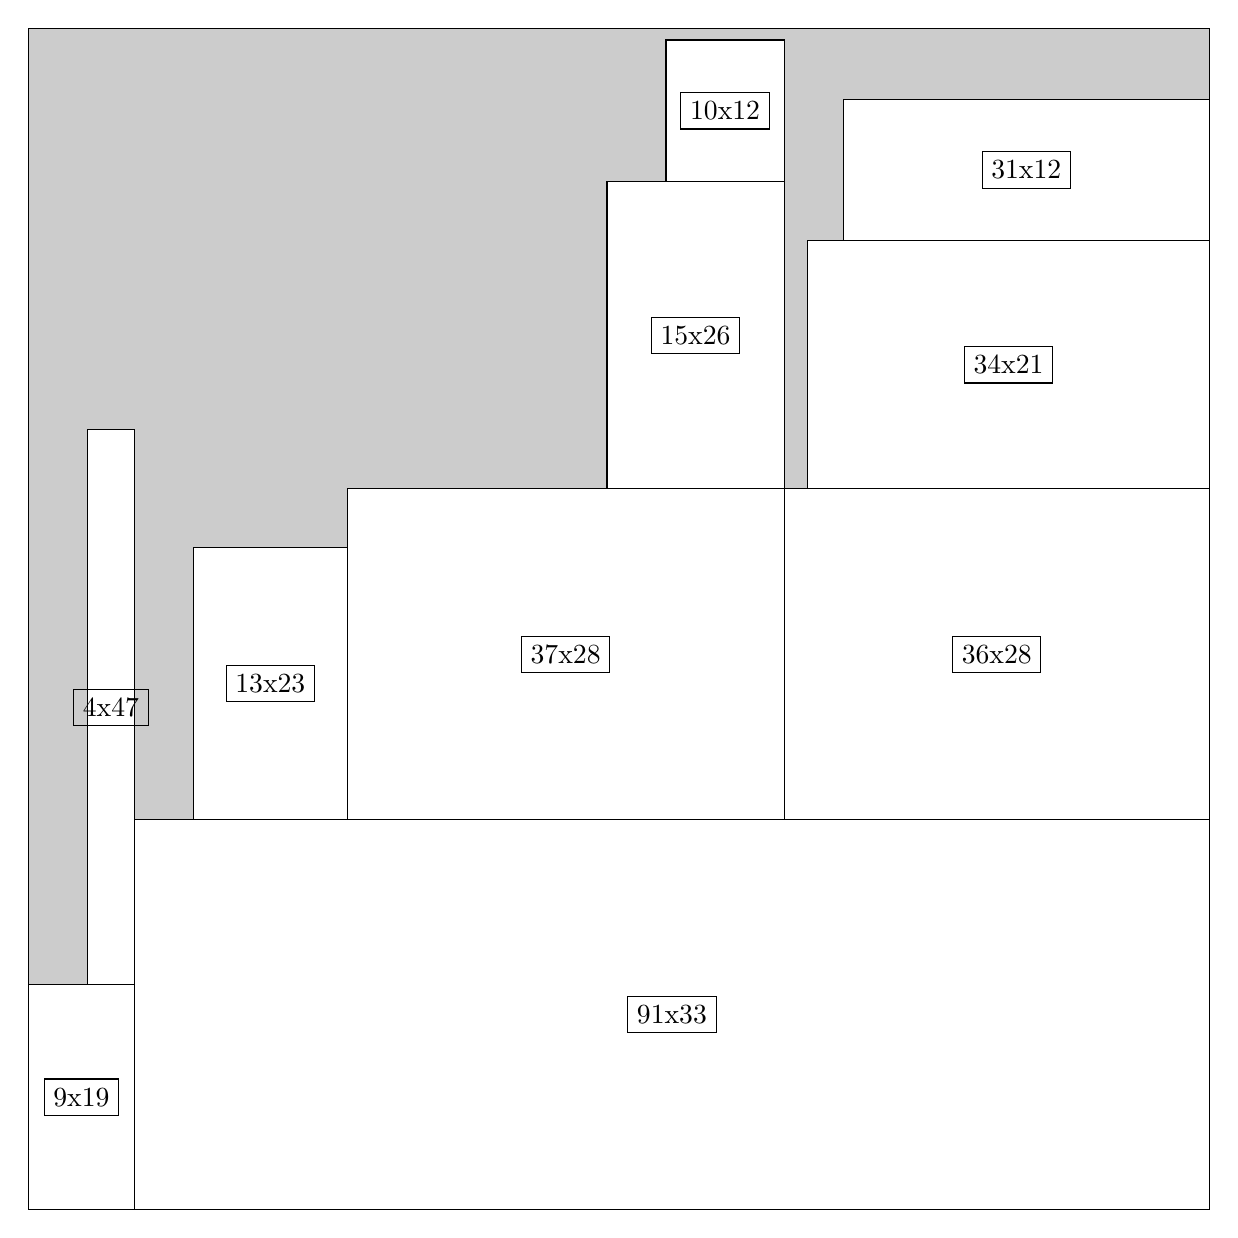
\begin{tikzpicture}[shorten >=1pt,scale=1.0,every node/.style={scale=1.0},->]
\tikzstyle{vertex}=[circle,fill=black!25,minimum size=14pt,inner sep=0pt]
\filldraw[fill=gray!40!white, draw=black] (0,0) rectangle (15.0,15.0);
\foreach \name/\x/\y/\w/\h in {91x33/1.3499999999999999/0.0/13.65/4.95,36x28/9.6/4.95/5.3999999999999995/4.2,34x21/9.9/9.15/5.1/3.15,31x12/10.35/12.299999999999999/4.6499999999999995/1.7999999999999998,37x28/4.05/4.95/5.55/4.2,13x23/2.1/4.95/1.95/3.4499999999999997,15x26/7.35/9.15/2.25/3.9,10x12/8.1/13.049999999999999/1.5/1.7999999999999998,9x19/0.0/0.0/1.3499999999999999/2.85,4x47/0.75/2.85/0.6/7.05}
\filldraw[fill=white!40!white, draw=black] (\x,\y) rectangle node[draw] (\name) {\name} ++(\w,\h);
\end{tikzpicture}


w =91 , h =33 , x =9 , y =0 , v =3003
\par
w =36 , h =28 , x =64 , y =33 , v =1008
\par
w =34 , h =21 , x =66 , y =61 , v =714
\par
w =31 , h =12 , x =69 , y =82 , v =372
\par
w =37 , h =28 , x =27 , y =33 , v =1036
\par
w =13 , h =23 , x =14 , y =33 , v =299
\par
w =15 , h =26 , x =49 , y =61 , v =390
\par
w =10 , h =12 , x =54 , y =87 , v =120
\par
w =9 , h =19 , x =0 , y =0 , v =171
\par
w =4 , h =47 , x =5 , y =19 , v =188
\par
\newpage


\end{document}